\section{Configuration Characteristics}

Prior research in computer networking hints that we should expect network configurations to share a common set of tokens~\cite{compelxity}. We took configurations from a large university network and split up each configuration file into a list of tokens. Tokens included all keywords and subnets with punctuation and newline characters stripped off. For every file we then plotted the percentage of tokens that exist in other router configuration files (Figure~\ref{fig:chart}).\\

\begin{figure}
	\centering
	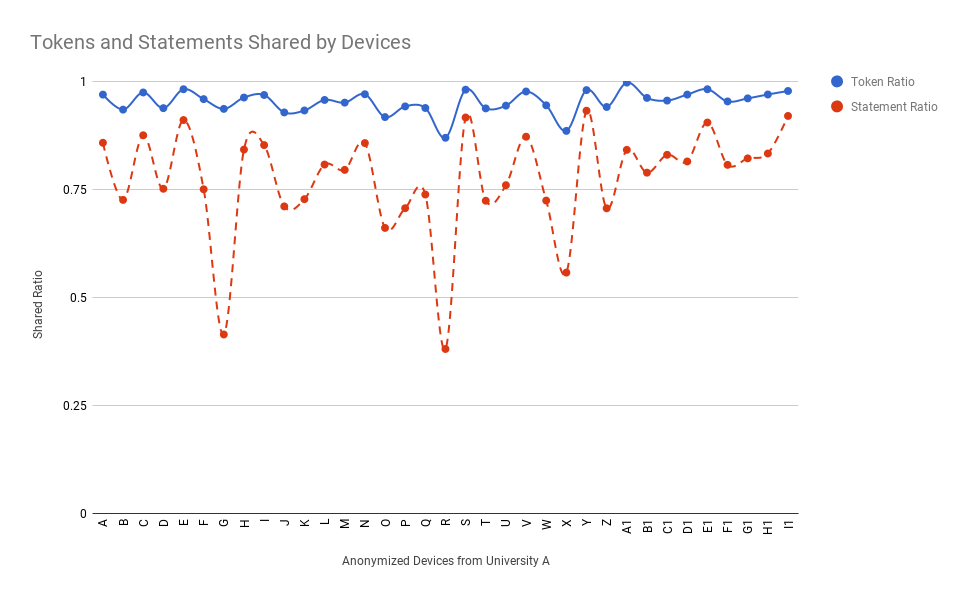
\includegraphics[width=\columnwidth]{chart.png}
	\caption{The plot shows how many tokens and statements a router configuration holds in common with the rest of the network. The data was taken from a large research university.}
    \label{fig:chart}
\end{figure}

Our results show that all most all configurations could be rebuilt from the same set of unique tokens. However, the same configuration files may not share all the statements that appear in other routers in the networks indicating that some routers are configured differently. Given our results, and the observations made by~\cite{complexity} about how networks are configured, we can confidently hypothesize that most token suggestions can be generated from analyzing other existing configurations.\\


\section{NLP-based Configuration Completion}

Now that we have confirmed the notion of regularity in our configurations, we can start using statistical techniques to our advantage. According to Hindle,\textit{et al.} 2012~\cite{naturalness}, regularities in bodies of texts can be easily exploited by NLP techniques. Inspired by them, we decided to use N-grams as a basis of our model. This effectively makes all router configuration histories a part of the search space for our model. We use an N-gram model to generate predictions using likelihood estimators to score our n-grams. In particular, we made use of bigrams and trigrams, the latter of which performed consistently better. We preprocessed the data and added placeholders for certain tokens like IP addresses, subnet masks, and interface names.\\
\begin{figure}
	\centering
	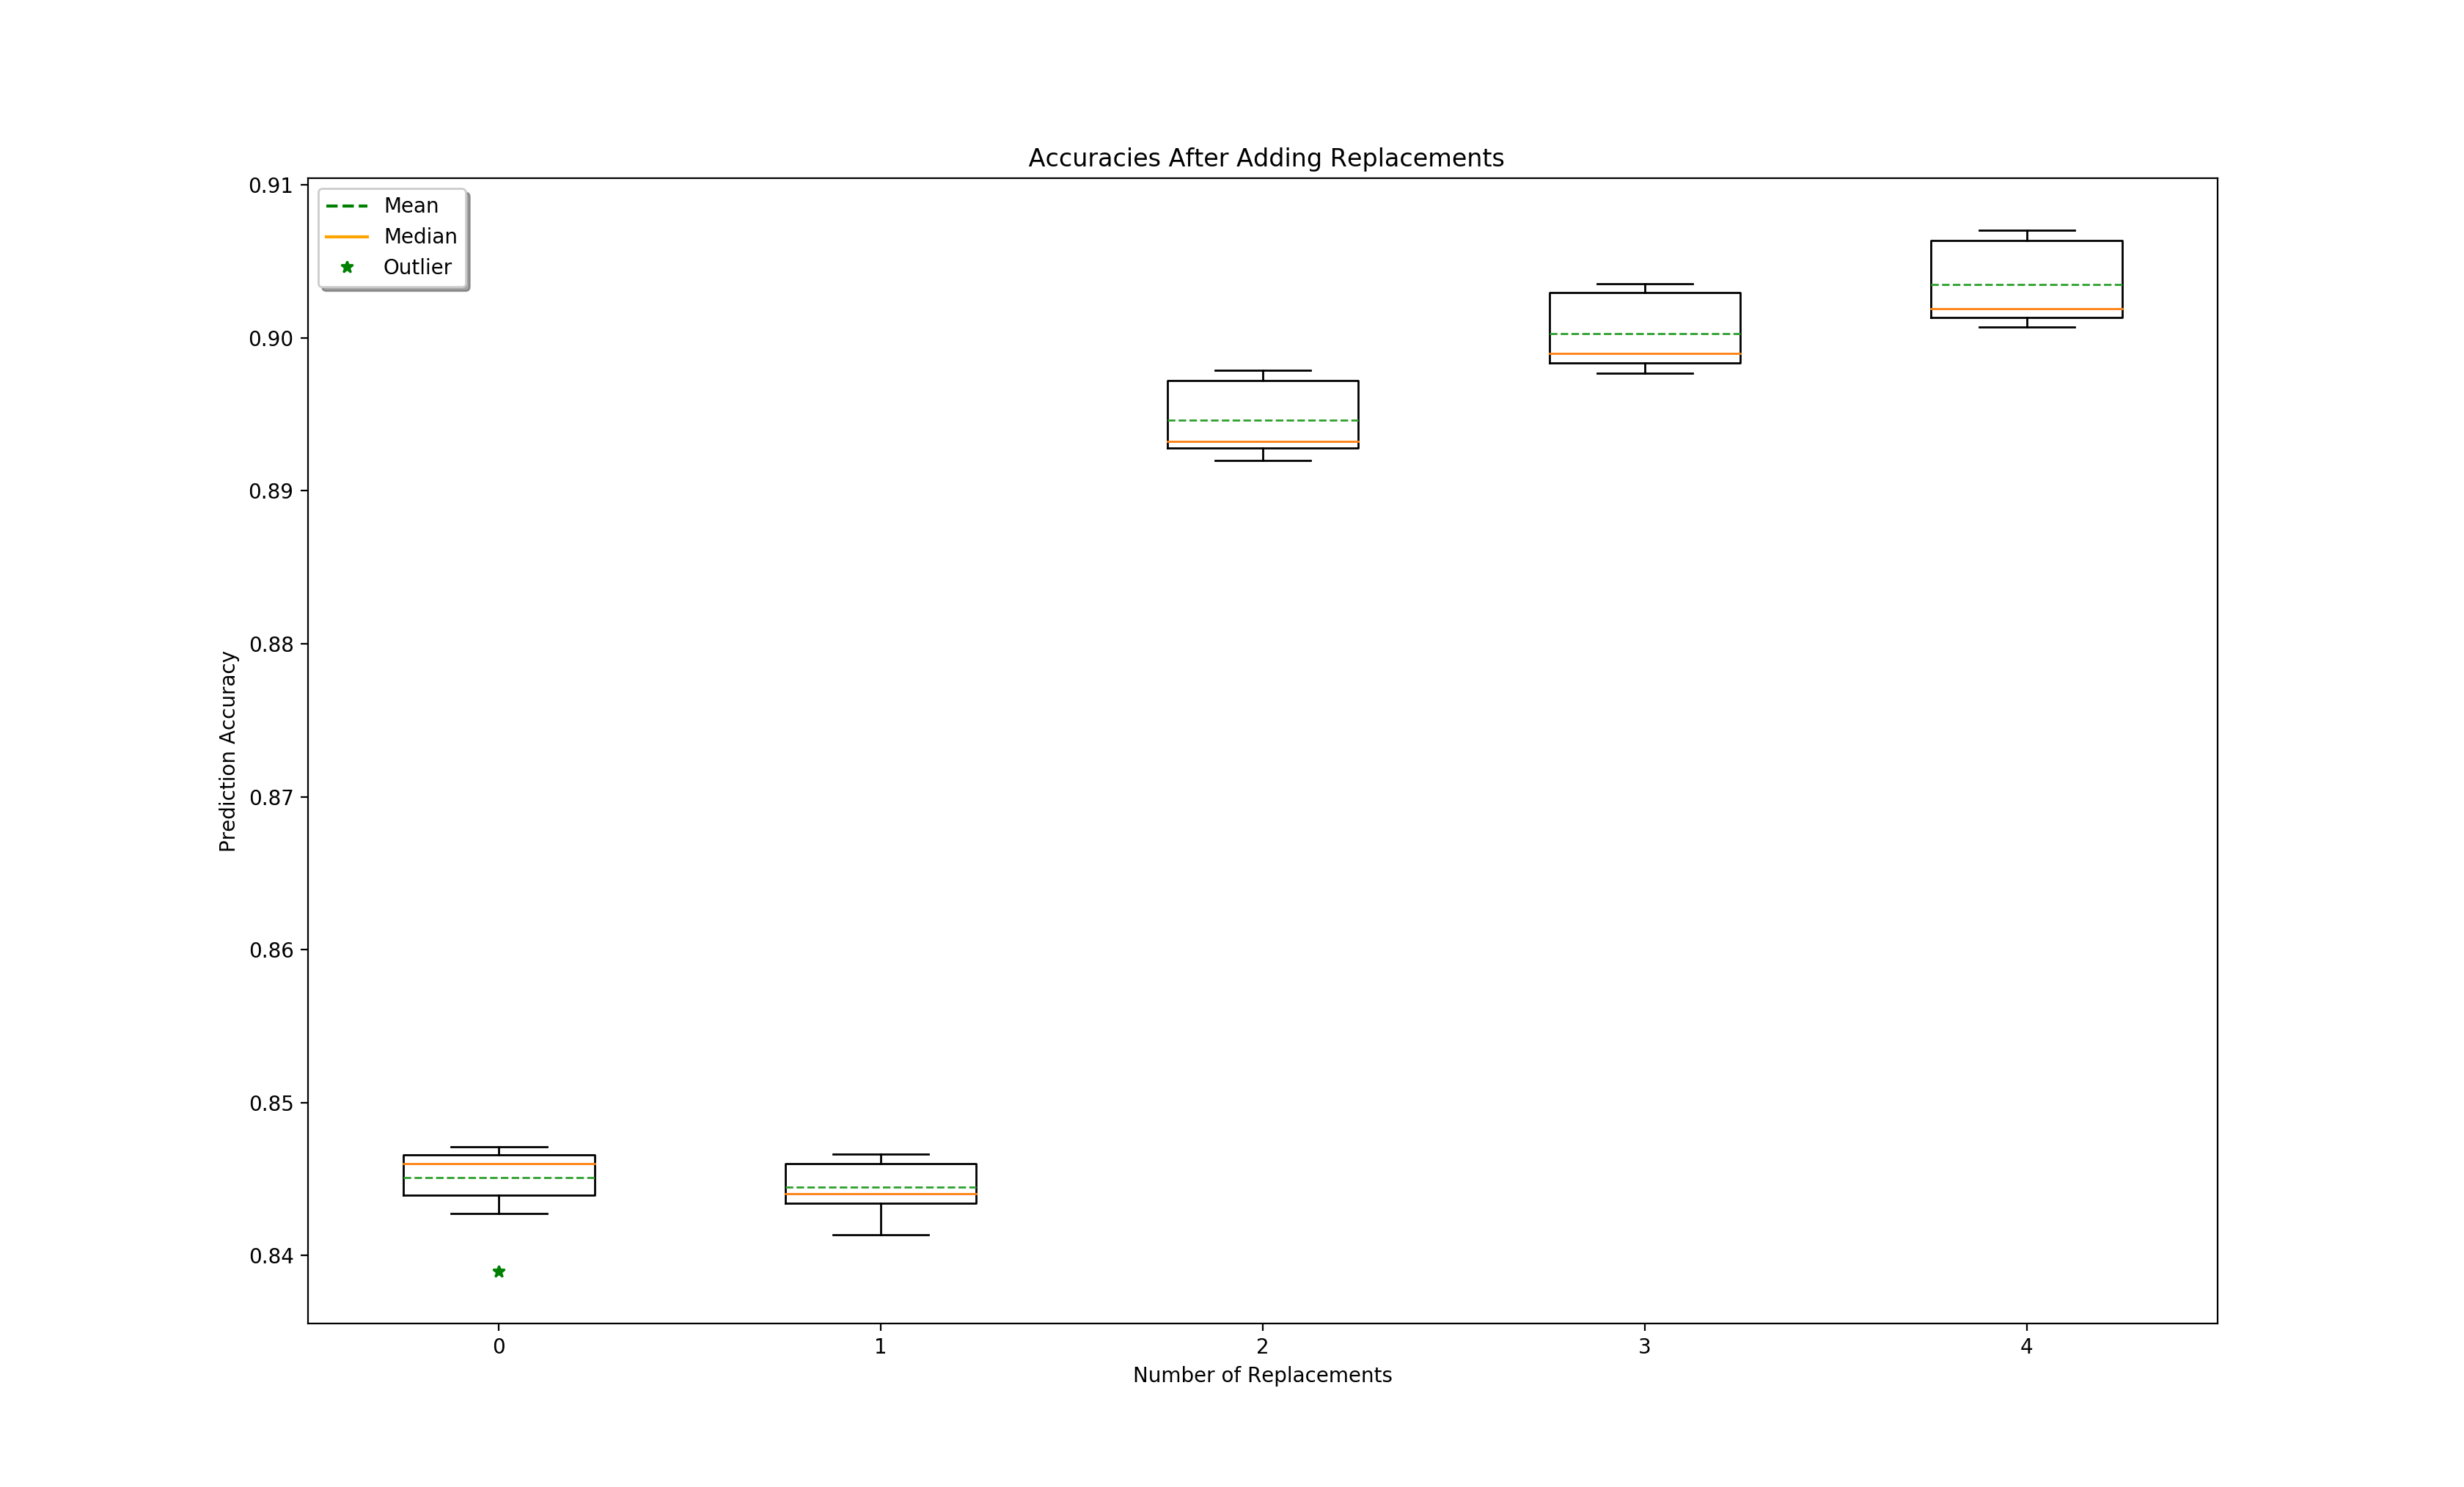
\includegraphics[width=\columnwidth]{replacement_analysis.png}
	\caption{Accuracy increase as we utilize placeholders to replace noisy tokens}
    \label{fig:replacement_analysis}
\end{figure}

\subsection{Preliminary Results}

We analyzed three large university networks, with configurations retrieved form core routers, border routers, and distribution switches. All the routers belong to CISCO and are therefore the configurations are written using the CISCO's language. Universities A, B, and C have 35, 26 and 24 routers respectively


\begin{center}
    \begin{tabular}{ | p{1.5cm} | p{1.5cm}| p{2cm} |  p{1.5cm} |} 
    \hline
    University & Number of Configurations & Average Unique Statements & Average Unique Tokens \\ \hline
    A & 11C & 22C &1000 \\  \hline
    B & 26 & 526 & 608  \\ \hline
    C & 24 & 606 & 750\\  \hline
    \end{tabular}
\end{center}

(Figure~\ref{fig:uni_analysis}). Next, we analyzed the effects of sampling more configuration in time (Figure~\ref{fig:time_analysis}), which did not seem to have a statistically relevant effect on our accuracies. We also varied the number of devices considered for our training set (Figure~\ref{fig:device_analysis}). This helped us assess our model's performance when we considered devices with different roles. Additionally, our analyses showed that our preprocessing helped reduce a significant amount of noise from the data, where we saw a 5\% increase in accuracy through placeholders alone. The majority of this increase came through generalizing IP addresses and subnet masks.\\

\begin{figure}
	\centering
	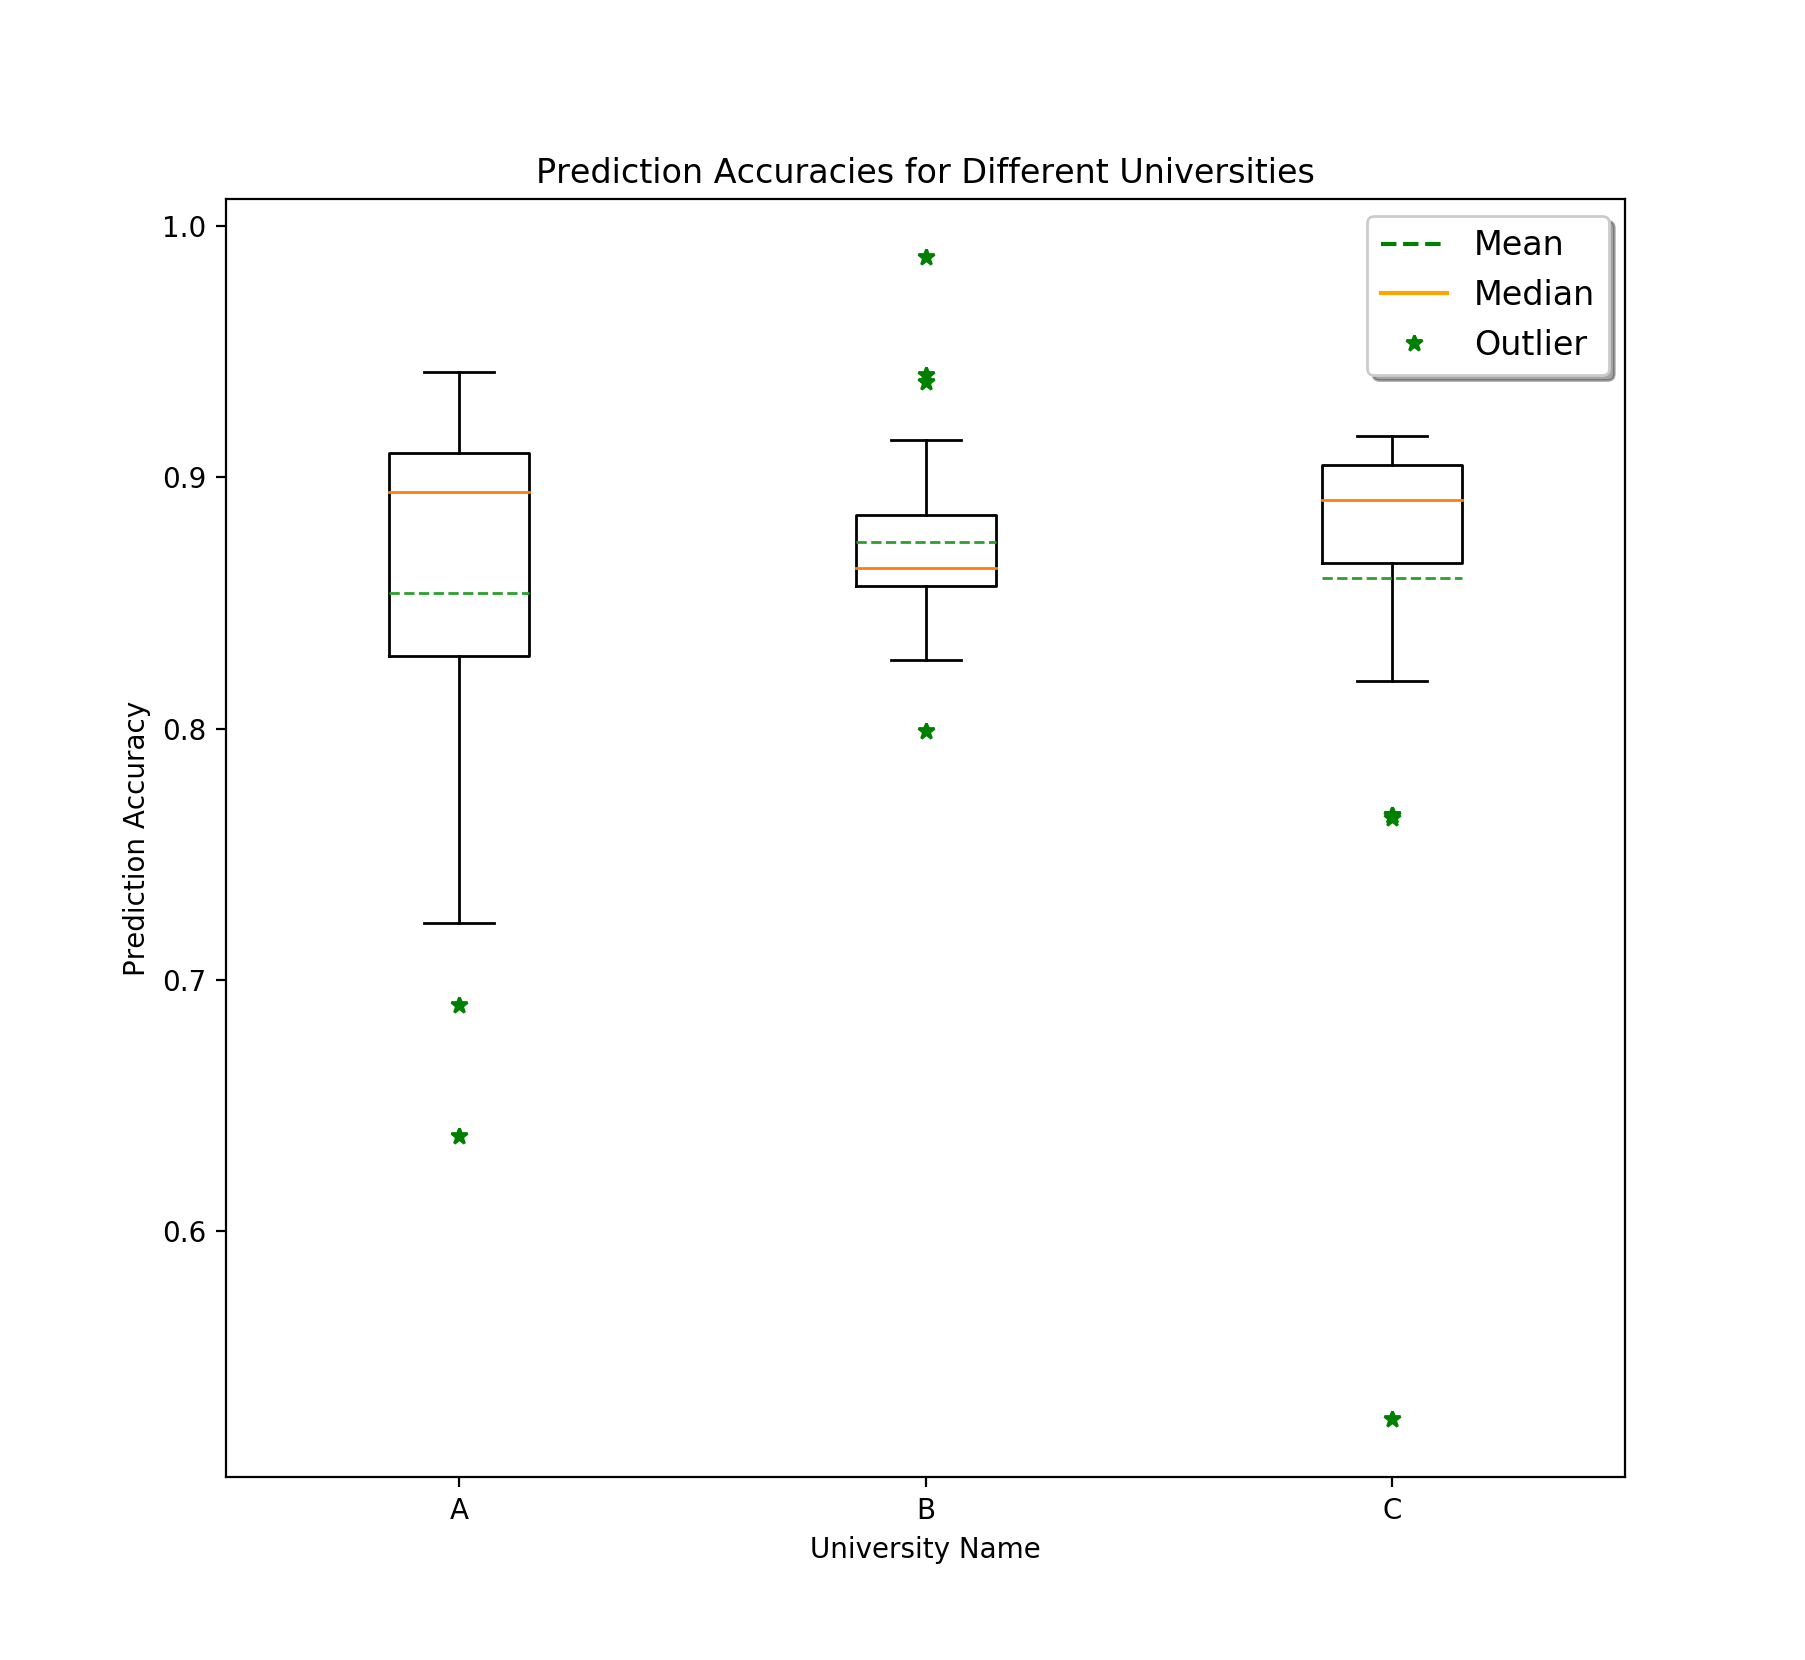
\includegraphics[width=\columnwidth]{uni_analysis.png}
	\caption{Some universities may have routers for different roles, causing more outliers.}
    \label{fig:uni_analysis}
\end{figure}

\begin{figure}
	\centering
	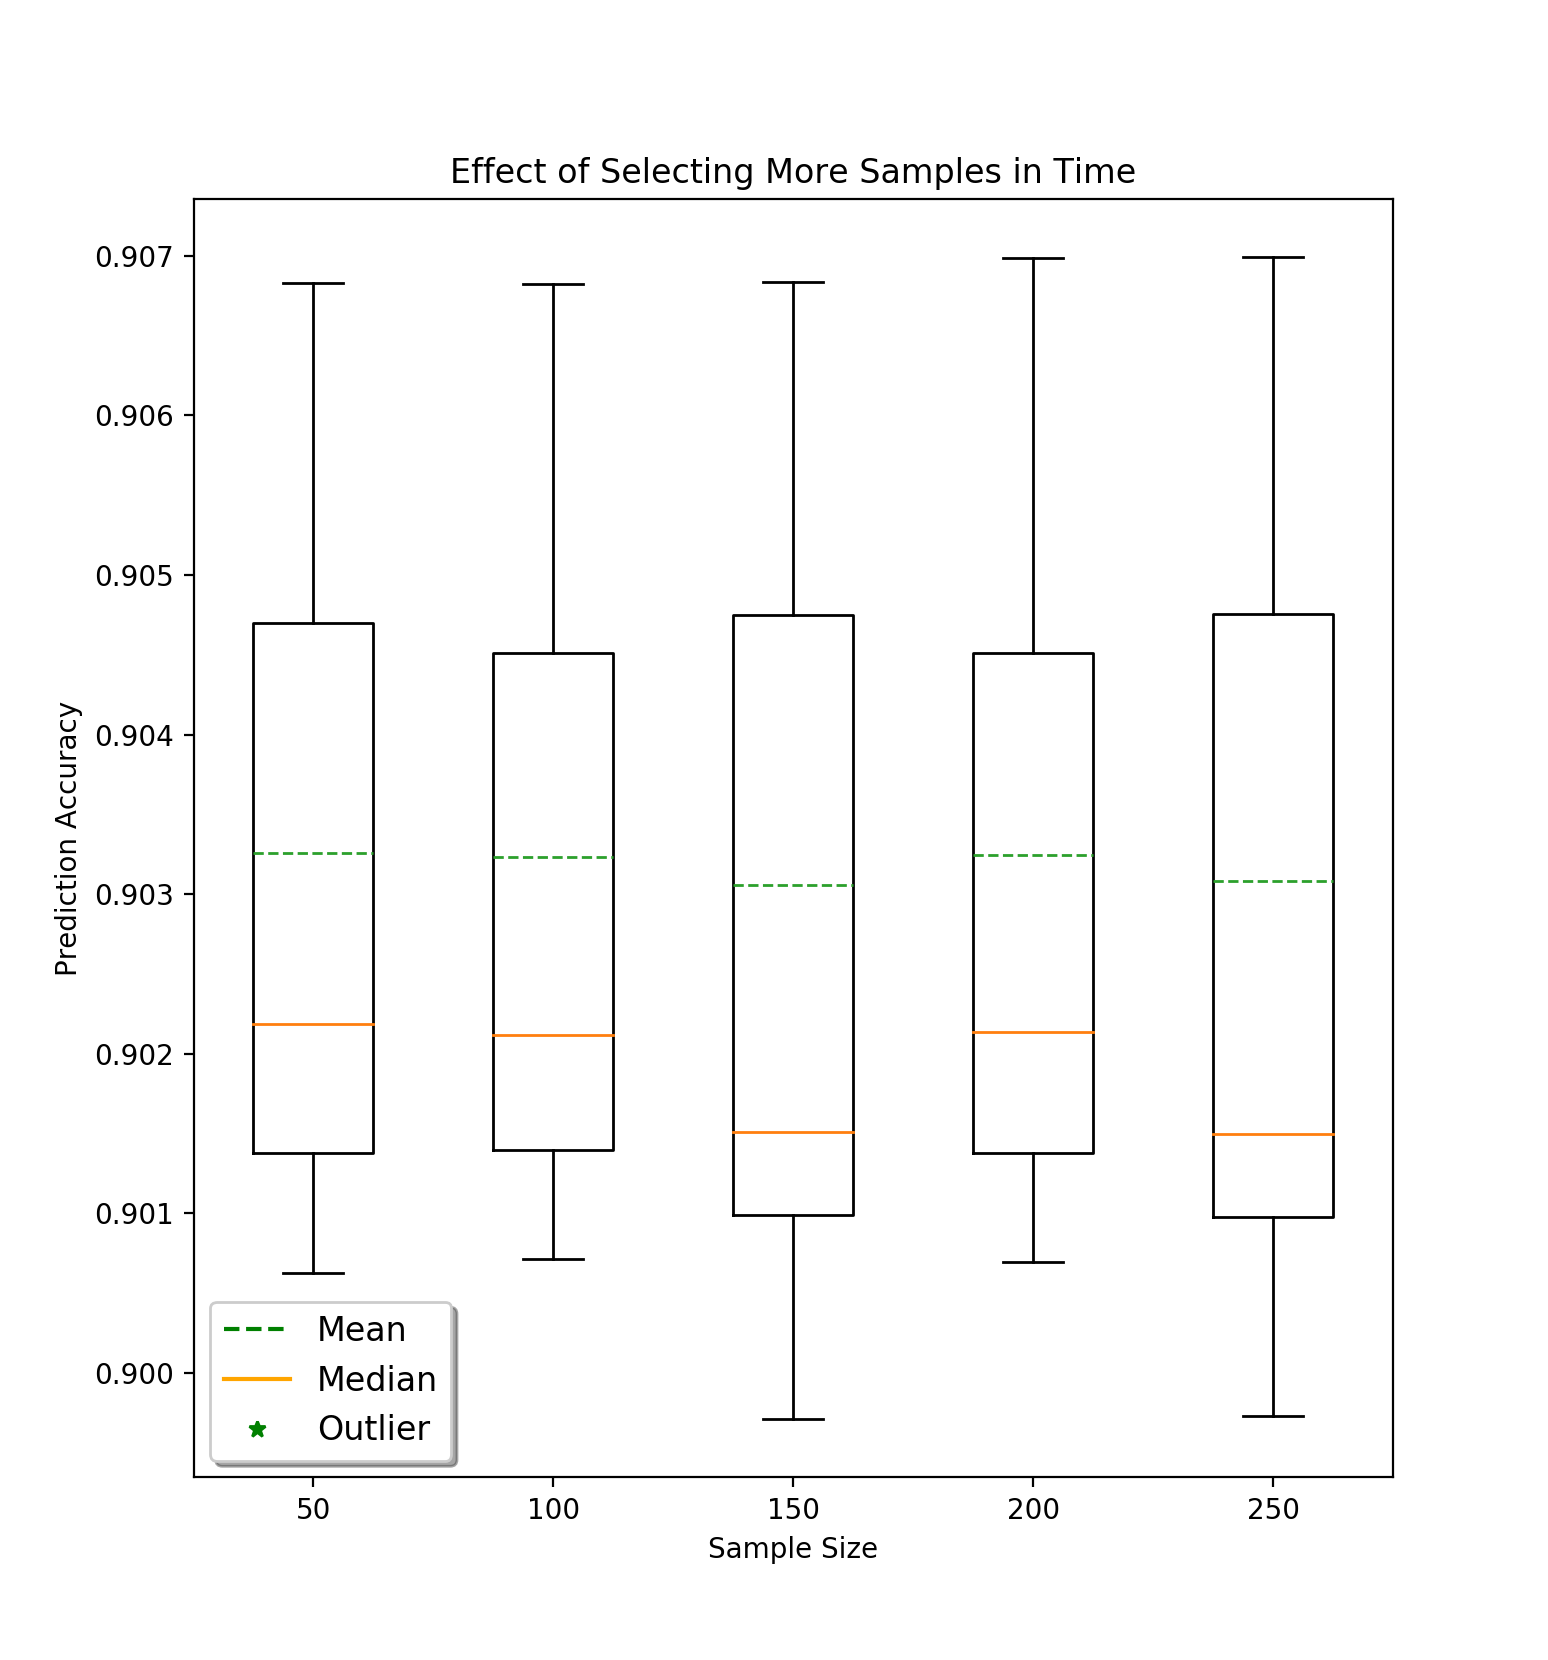
\includegraphics[width=\columnwidth]{time_analysis.png}
	\caption{Increasing the number of samples did not have any statistically significant affect on prediction accuracies}
    \label{fig:umn_analysis}
\end{figure}

\begin{figure}
	\centering
	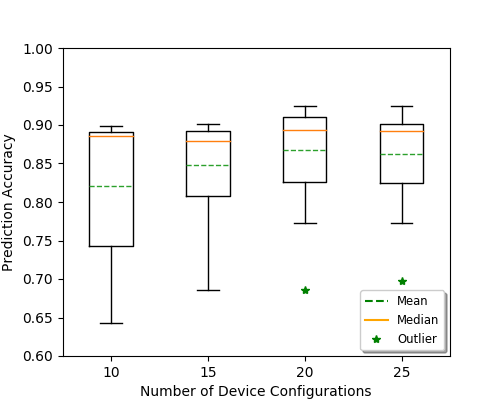
\includegraphics[width=\columnwidth]{device_analysis.png}
	\caption{Accuracies generally increase as more devices are considered, until a saturation point is reached after which the types of devices being added start playing a more important role}
    \label{fig:umn_analysis}
\end{figure}

To test the accuracy of our model, we perform Leave One Out (LOO) Cross Validation. This form of cross validation involves using one observation as the validation set and the remaining observations as the training set. Our program will "walk through" rebuilding a test configuration (A), starting from the first keyword. At every step, we invoke our n-gram model to predict a token using n-1 tokens that came before it. We then compare our predictions against the actual tokens in the test configuration. A prediction is marked as successful when the correct token lies within the top three results generated by the model. Our initial analyses showed that the engine was trying to predict what the user would enter after a complete configuration statement. This greatly affected our accuracies, and thus we altered our model to only suggest tokens that appear on the same line.\\

\section{Future Work}

Our analyses help direct our attention towards areas of improvements for the model. The variance seen in our device analysis suggests that having different models for router of different "roles" could help improve prediction accuracies. Additionally, we plan on exploring the possibility of using larger n-grams to suggest complete statements. Lastly, we hope to evaluate our model against the current state of the art: tab-completion in CLIs on modern routers.